\chapter{Basic machine learning principals}

%
% Discuss the basics of what a machine learning algorithm is
%
In this chapter I will explain some of the basic underlying
principals of machine learning techniques including: 
fully-connected neural networks, \ac{CNN}s 
and \ac{CVAE}s. I will also 
describe some of the basic principals of how neural networks 
learn (e.g. backpropogation), how they are initialized, 
best training practices, methods for evaluating performance, 
and methods for data augmentation/processing.

First off, to dispel any notion of machine learning being 
thought of as black magic, machine learning is nothing more 
than statistics and function approximation at the end of 
the day. The overarching goal being to approximate a 
function which is trained to find a global minimum 
(though this rarely is the case in reality and most 
often a local minimum will suffice). How one defines 
this minimised function is the name of the game and there 
are many methods for doing so. 

A machine learning algorithm can perform many useful tasks 
such as: classification, regression, anomaly 
detection, denoising and density estimation. Of course, 
there are many other tasks a machine learning algorithm 
can tackle, but the three which are primarily used in this 
thesis are classification, regression and density estimation.
In classification, a machine learning algorithm attempts 
to learn the optimal function to classify a given set 
of inputs (e.g. a time series or image) and returns as 
output the likelihood that the given input came from a 
particular class or set of 
classes. A machine learning algorithm can also perform 
non-linear regression by instead of outputing numeric 
values describing class probability, we have the algorithm 
predict a continuous variable. Finally, we can even have a machine learning 
algorithm produce probability distributions for a given 
input (e.g. gravitational wave source parameter posteriors) by 
making the algorithm predict moments which describe 
such a distribution. 

\section{Introduction to fully-connected neural networks}

%
% The perceptron and deep neural networks
%
So, how do we build a machine learning algorithm? Before making things too complicated lets first define a simple neural network architecture, the perceptron. A perceptron is made up of one neuron which takes a set of inputs from a trainig sample and outputs a prediction given that training sample (illustrated in Fig. \ref{fig:Perceptron_network}). For the sake of simplicity lets presume we want to perform a binary classification task. The perceptron can be defined as a learned function

\begin{equation}
    z = \sum_{i=1}^{N} w_{i} x_{i} + b
\end{equation}{}

\begin{equation}
    y_{p} = \sigma(z),
\end{equation}{}

\begin{figure}
    \centering
    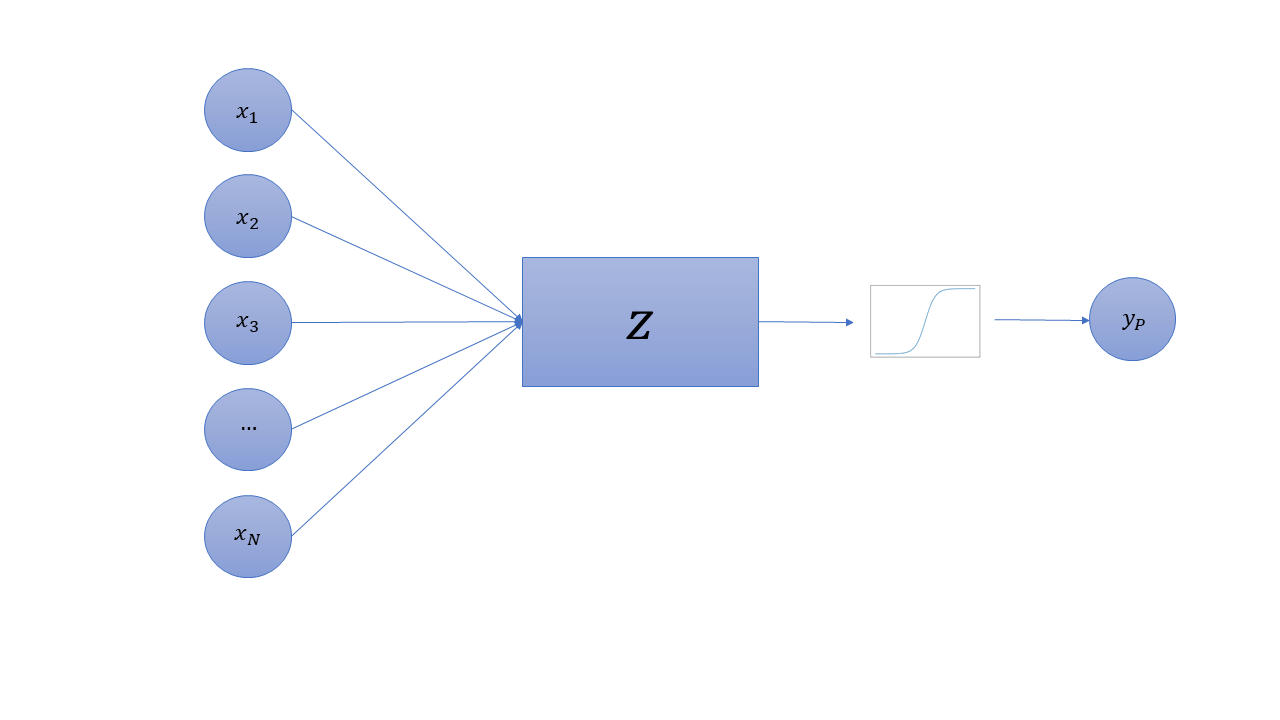
\includegraphics[width=\linewidth]{figures/Perceptron_network.png}
    \caption{A perceptron network whose inputs $x_1 ... x_N$ are each multiplied 
    by a learned set of corresponding weights $w_1 ... w_N$ and summed together in $z$. 
    The summed value is then passed through an activation function to get the final 
    output of the network.}
    \label{fig:Perceptron_network}
\end{figure}

where $y_{p}$ is our predicted output (e.g. class label), $x$ is our given input, $w$ is a learned scalar weighting term on $x$, $b$ is a learned scalar bias term on $x$ and $\sigma$ is a nonlinear activation function (Fig. \ref{fig:sigmoid}) which rescales the output.

\begin{figure}
    \centering
    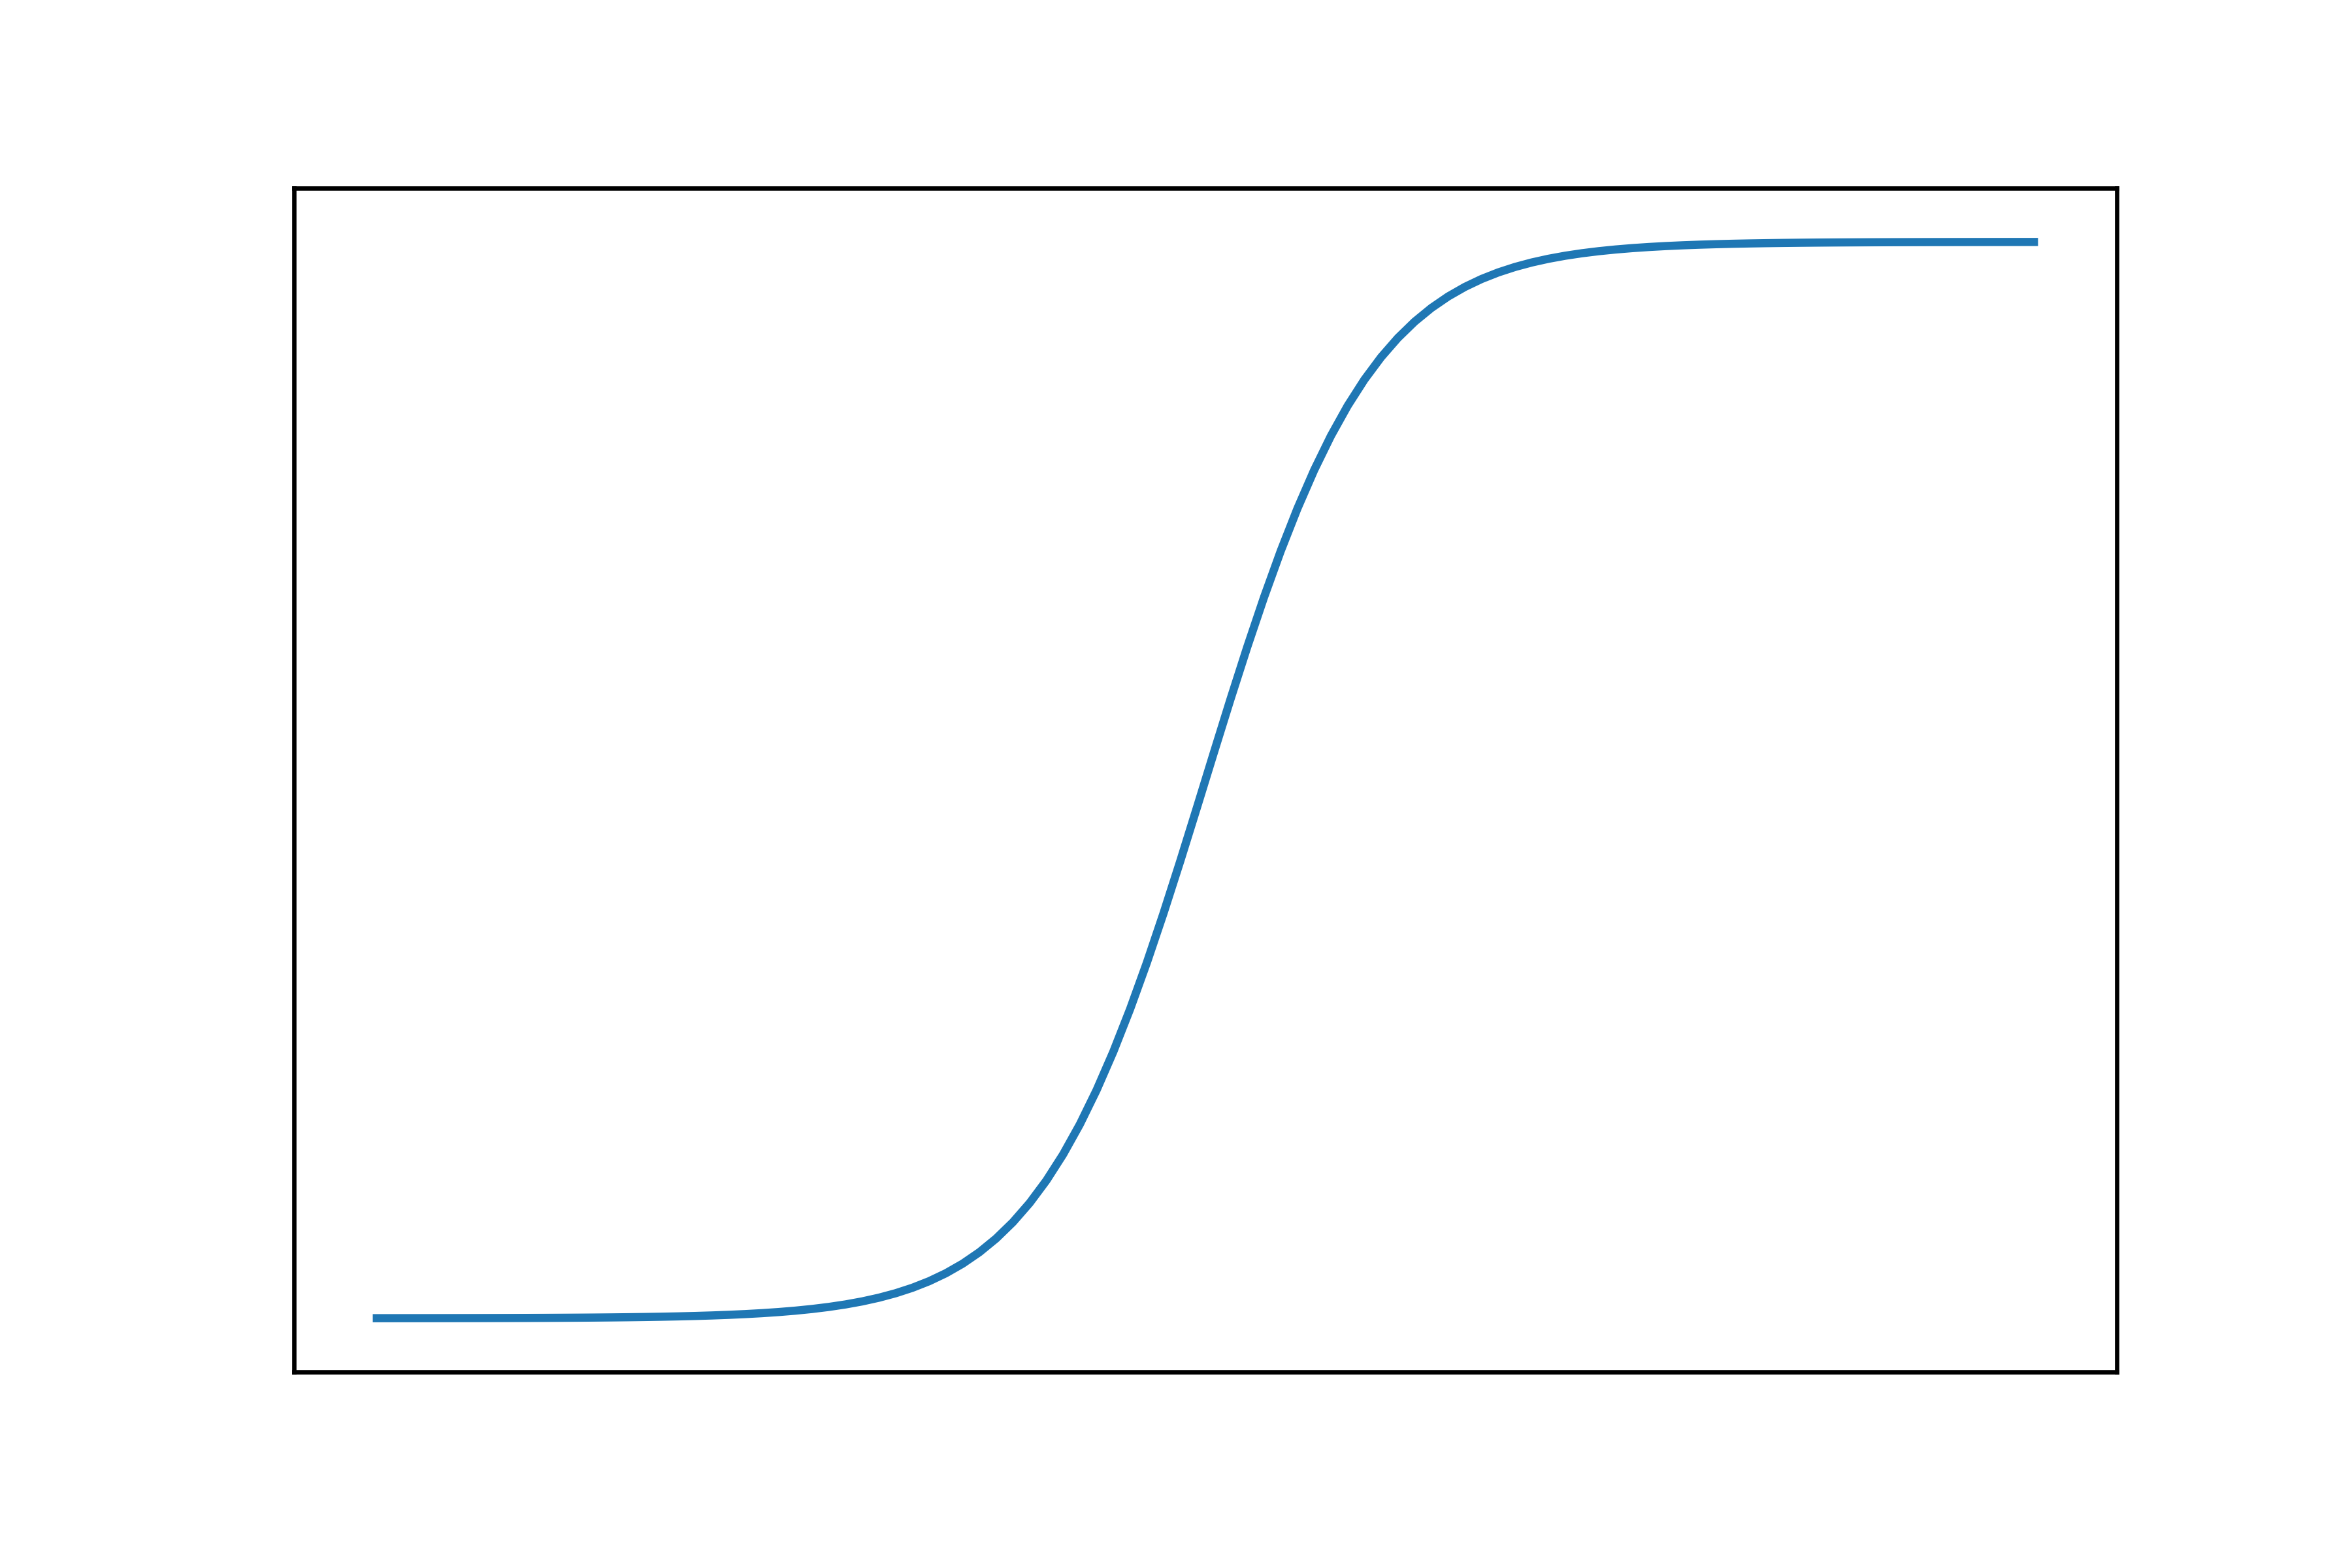
\includegraphics[width=\linewidth]{figures/sigmoid_function.png}
    \caption{A sigmoid activation function plotted over the input 
    range -10 to 10. Given an input over a pre-defined range, the 
    activation function will rescale the input to be between the range 
    of 0 to 1.}
    \label{fig:sigmoid}
\end{figure}

We apply a nonlinear activation function in order to allow our perceptron to learn non-linear functions/features. All weights and biases are typically initialized randomly prior to training and there are many formalisms for choosing the optimal initialization. In order to approximate more complicated functions, we can string together multiple perceptrons (neurons) in a layer where each neuron is fully-connected to the given input $x$ (i.e. every element in our input is multiplied by each weight of each neuron in our first layer). To make a deep network, we can randomly initialize another layer of neurons (of arbitrary size) which takes as input the output from the previous first layer of neurons (illustrated in Fig.\ref{fig:deep_nn}). Additional layers can be added in perpetuity. During training, weights and biases are updated according to the performance of the algorithm with respect to a loss function which describes how well the algorithm is performing with respect to the true value of each training sample. This loss function can take many forms, but most often a mean squared error is used

\begin{figure}
    \centering
    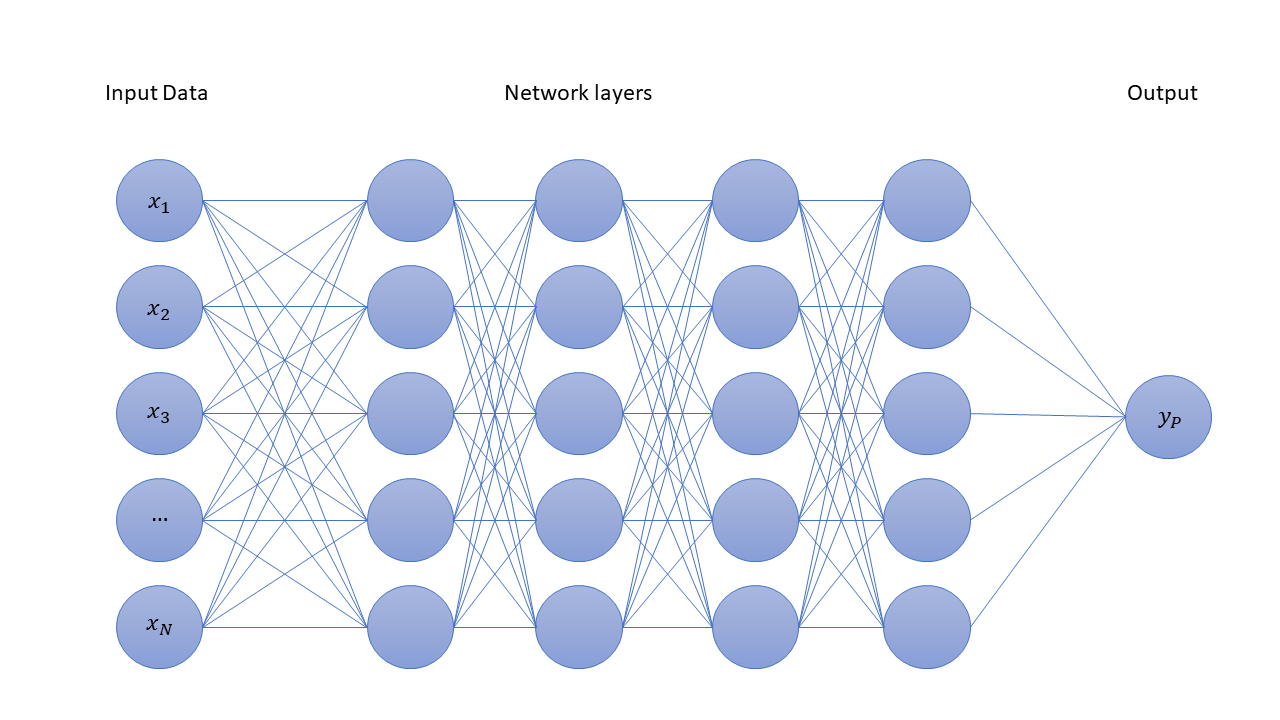
\includegraphics[width=17cm,height=20cm,keepaspectratio]{figures/DeepFullyConnectedNetwork.png}
    \caption{A deep fully-connected neural network. Inputs $x_1 ... x_N$ are given as input to the 
    first layer of the neural network and are fully-connected to every node in that layer. The outputs 
    of each node are then passed on to the next set of nodes in the next layer and are also fully-
    connected. The final layer passes through a final single node which determines the class/value 
    of the given input.}
    \label{fig:deep_nn}
\end{figure}

\begin{equation}
    L = \frac{1}{n} \sum_{i=1}^{n}(y^{l}_n-y^{t}_n)^2.
\end{equation}{}

%
% the loss function
%
When the predicted label of nth training sample in the final layer $l$ $y^{l}_n$ is the same as the nth training sample true label $y^{t}_n$, the loss term equals zero and is at a minimum. The reader's next question may rightly be, how does one go about choosing the right weights $w$ and biases $b$ for each neuron in the network? In other words, how much of an effect will changing $[w,b]$ have on the resulting loss function $L$. This may be accomplished through the use of gradient decent. Specifically, we will be discussing a variant of gradient decent, stochastic gradient decent.

% Hebian theory "neurons that fire together, wire together"
%
% Stochastic gradient decent explanation
%
Stochastic gradient decent is an iterative algorithm used to find the global minimum (usually a local minimum is sufficient) of a function. Gradient decent essentially has two decisions it needs to make when choosing new weights and biases: what direction to go and by how much. The most straightforward way of getting this information is through the use of a derivative, specifically the gradient of the loss function $L$ defined as 

\begin{equation}
    g = - \gamma \nabla L(y^{l}),
\end{equation}{}

where $\gamma$ is a tunable step size scale factor (typically called the learning rate), $\nabla L(y^{l})$ is the gradient of the loss with respect to the weights and biases of the network and $g$ is a list of gradients corresponding to each weight and bias between the final output layer and the previous layer. The sign of the gradient for each weight and bias corresponds to the direction of in which to change the weights while the magnitude tells you how sensitive the loss function is to each weight and bias. If there are multiple neurons in the final layer of the network, the contributing gradients for each neuron in the final layer are summed in order to return a representative gradient with respect to all output neurons.

However, this only returns the gradients for the final output layer. In  order to appropriately update weights and biases in the previous layers we must propagate the gradient backwards. This process is better known as back propagation.

%
% Back prop explanation
%
In back propagation we use the computed gradient from the final layer and compute the gradient between that final layer gradient and the output from the third to last layer. The individuals contributions from each neuron in the second to last layer are summed (same as was done in the final layer computation) and the gradients in the second to last layer are propagated back again to the third to last layer. Mathematically, we can define this process as the derivative of the loss with respect to the outputs of each layer $l$

\begin{equation}
    \nabla L(y^{l}) = \frac{\delta L}{\delta y^{(l)}}.
\end{equation}{}

Applying the chain rule and expanding this out for multiple layers we arrive at

% Need to add notation describing summation over each neuron in each layer
\begin{equation}
    \nabla L(y^{l}) = \frac{\delta z^{(l-m)}}{\delta y^{(l-m-1)}} \frac{\delta y^{(l-m)}}{\delta z^{(l-m)}} ... \frac{\delta z^{(l)}}{\delta y^{(l-1)}} \frac{\delta y^{(l)}}{\delta z^{(l)}} \frac{\delta L}{\delta y^{(l)}} 
\end{equation}{}

where the total derivative over all neurons in each layer may be quantified and applied to determine how much to shift each weight and bias in order to improve the overall loss of the neural network. This process is repeated until all weights and biases in the network have had their gradients computed. Ideally, we would compute the gradient over more than just one training sample, but rather the whole training set during each training iteration. However, computing the gradient over the whole network for all training samples is abhorrently expensive, so the training set is typically split up into mini-batches of samples in order to reduce the computational cost.

%
% Training best practices
%
\section{Training best practices (practical advice for the reader)}

I was commonly told when first wadding into the pool of deep learning that the practical implementation/training of deep learning models is largely a dark art. In this section, I would like to dispel that myth by offering some best practices when training any machine learning model.

%
% When in doubt, make more training data
%
First off, when in doubt, the more training data available to you, the better. Time and again, during a large part of my thesis work, we would spend countless hours tuning and tweaking our neural network architecture only to run up against some insurmountable wall of impeded progress. Only to increase the number of training samples by several factors and see a significant increase in performance. 

\subsection{Data pre-processing and augmentation}

\subsubsection{Data pre-processing}
Commonly, our input datasets are in a messy form. In order to help the network learn more efficiently, it is encouraged to perform some pre-procesing steps. It's important to do this because if our input data has large values over a wide range, and because our network is trying to learn a mapping from input to prediction, the learned weights may also end up being very large. Large learned variable weights can lead to massive gradients which cause the network to update weights in large step sizes, making the whole network more unstable in the process. We can overcome this by normalising our input dataset to be between the range of zero to one 

\begin{equation}
    y = \frac{x - x_{\textrm{min}}}{x_{\textrm{max}}-x_{\textrm{min}}},
\end{equation}

where $y$ is our new normalised data, $x$ is our original unnormalised data, $x_{\textrm{min}}$ is our unnormalised data minimum value and $x_{\textrm{max}}$ is our unnormalised data maximum value. It can also be advantageous to rescale our input data to a standard normal distribution if our data has widely varying scales by applying 

\begin{equation}
    y = \frac{x - x_{\textrm{mean}}}{x_{\textrm{std}}},
\end{equation}

where $x_{\textrm{mean}}$ is the mean of our data and $x_{\textrm{std}}$ is the standard devitation of our data. In addition to rescaling our input data, we ocassionally need to also rescale our training labels. This is especially relevant if the activation function in our final neural network layer is fixed to be between some values. For example, if we were using a sigmoid activation function where the values of the output of the sigmoid are only allowed to be between zero and one, then we would also want our training label values to lie between zero and one since the network would not be able to produce values outside of that range.

\subsubsection{Data augmentation}

Neural networks can sometimes be composed of hundreds, thousands, even million of parameters to be tuned during training. Given the massive number of parameters, many complex networks require an equally massive number of training samples. But, what do you do if you are only given a limited number of training samples? This is where data augmentation comes to the rescue. In order to generate more training data, we can apply simple shifts to the existing limited dataset and greatly expand the number of training samples. This can be accomplished through many of the following methods:

\begin{itemize}
    \item Translation: Shift the input data sample in the x/y/z direction.
    \item Rotation: Rotate data about a fixed point.
    \item Cropping: Choose a random subset of the input sample, cut out all data outside of subsection, rescale cropped data to original input size.
    \item Gaussian noise: Add varying amounts of Gaussian noise in order to simulate poor quality signals.
\end{itemize}

%
% The purpose of Validation
%
\subsection{Validation}
In order to understand how well your model is performing with respect to the training data, one may plot the resultant average output of the loss function as a function of the number of training iterations. Ideally, we would like the loss to rapidly decrease and to then flatten out. Although this will give us an indication of how well the network is performing on the training set, it does not inform us as to how well the model will generalize to a novel testing set. In order to quantify the generalization ability of the network, we may set aside a small portion of the training set prior to training as a validation set. During training, we can temporarily freeze the weights and run the validation set through the model in order to compute a validation loss. 

If we plot both the validation loss and the training loss as a function of time, we again ideally would like to see both curves decrease as a function of training iteration and then level out. However, if we see that the training curve initially decreases and then continues to decrease while the validation curve initially decreases and then subsequently increases we may say that the model has overfit the training data. Overfitting the training set generally indicates that either our model is too complicated and has essentially memorized the training the set or that we do not have enough training data to sufficiently cover the entire parameter space. 

If on the other hand we see that the validation loss decreases far quicker than the training loss then we may say that the model has underfit the data, which is generally an indication that the model needs to have an increased capacity.

%
% Regularization techniques
%
\subsection{Regularization}

%
% Dropout
%
Regularization is used to help prevent a machine learning model from overfitting the the training data. One of the easiest regularization techniques to implement is that of dropout. Dropout may be implemented across most types of neural network layers (i.e. fully-connected, convolutional filters, etc.) and rarely have any adverse effect on training. During training, if dropout is implemented a subset of the neurons in a layer will be switched off and not used when the gradient is computed and backpropogated through the network for a given training iteration. The percentage of neurons in a layer to switch off is a tunable parameter, though typically it is best to set a value of no more than $50\%$. Dropout effectively forces the neurons in a dropout layer to be able to identify multiple features, rather than to focus a small subset.

%
% Batch noramlization
%
Batch normalization is motivated by the same principle that standard normalization of input to a neural network is motivated. We want to reduce the space over which the neural network has to search. As such, batch normalization is essentially a normalization of the output of individual layers within a neural network to be between zero and one. This normalization prevents weights or biases from becoming too large. It is computed by normalization of the current layer according to the mean and standard deviation of the output of the previous layer and the subsequent rescaling through two learned variables ($\alpha$ and $\beta$) and is formalised as 

\begin{equation}
    z_n = \alpha \hat{z}_n + \beta,
\end{equation}{}

where $\alpha$ is a learnable parameter, $\beta$ is a learnable parameter and $\hat{z}_n$ is calculated by 

\begin{equation}\label{eq:batch_norm}
    \hat{z}_n = \frac{1}{n} \sum_{i=1}^{n} \frac{z_n - \mu}{\sigma^{2} + \epsilon},
\end{equation}{}

where $z_n$ is the output of the neural network layer summed over all outputs in the batch of that layer, $[\mu,\sigma]$ are the mean and standard deviation respectively of the batch of previous layer outputs introduced to the network and $\epsilon$ is a small constant. If it turns out that the application of batch normalization is not optimal, then the network may undo the above normalization in e.q. \ref{eq:batch_norm} through the optimization of $[\alpha,\beta]$ in each layer.

\subsection{Hyperparameter optimization}

Many instances, after we have spent all the time cleaning our data, 
choosing a model to solve our problem and then finally 
training our model, we find that the most tedious and 
time consuming part of the whole endeavor is all those 
pesky model hyperparameters. In this sub section, I will 
describe three approaches used in this thesis to optimize 
hyperparameter choices.

\subsubsection{Random Search}
Probably the simplest of the three approaches random search 
seeks to choose model hyperparameters based off of a 
predefined prior distribution for each hyperparameter. 
The user may define whatever distribution they prefer 
whether that be a multivariate Gaussian distribution 
or a uniform distribution so long as the bounds of the 
distribution chosen are within reason.

\subsubsection{Grid Search}

Grid search is marginally more complicated. In a grid 
search approach we define both an upper and a lower limit 
for each hyperparameter. Additionally, we define a step 
size by which we will increase the the hyperparameter 
value after each model evaluation (much like steps 
on a ladder). Each of these hyperparameter 
ladders are iterated over in an N dimensional grid, 
where N is representative of N hyperparameters 
describing the model. 

\subsubsection{Gaussian Process Bayesian hyperparameter optimization}

Bayesian hyperparamter optimization aims to minimize (or maximize) some 
objective function. In this case, we aim to learn an 
approximate surrogate model for an objective function which 
describes the loss function space and to minimize the value of the 
loss function output. The dimensionality of the search space 
is parameterized by the number of neural network hyperparameters being optimized 
and does not usually perform well past 20 dimensions. Gaussian process 
regression is used in order to minimize the uncertainty on the surrogate model estimate 
. We then use an acquisition function to sample from the approximate 
surrogate model to determine the next set of hyperparameters to use 
during the next round of neural network training \cite{1807.02811}.

In practice, we first choose an initial set of hyperparameters 
to use in order to train the network. This can either be randomly chosen 
from a reasonable prior, or a best guess from the practitioner. 
Next, the neural network is trained a pre-defined number of 
training iterations and the network loss function output value 
is given as input to the Bayesian optimization algorithm. The Bayesian 
optimization algorithm then updates its surrogate model 
based off of this new loss value from the neural network 
given the hyperparameters used and a new set of 
hyperparameters is chosen by an aquisition function based 
informed by the Gaussian process regression surrogate model. 
The above process is repeated for N user pre-defined iterations.
%
% Note, fill out this section using the following resources:
% https://arxiv.org/pdf/1807.02811.pdf
% https://towardsdatascience.com/tl-dr-gaussian-process-bayesian-optimization-5e66a014b693

\section{Convolutional Neural Networks}

\ac{CNN}s were first made popular in the late 1980s to early 1990s 
and one of the most famous examples is that of the LeNet archetecture 
made by Yann LeCunn in 1998 \cite{726791}. In his paper, LeCunn 
illustrated that \ac{CNN}s outperformed other simpler 
techniques like K Nearest Neighbor and fully-connected 
neural networks on a variety of image recognition 
tasks. In recent years \ac{CNN}s have been applied to 
many more domains including image object detection, 
fraud identification, healthcare analysis and many 
others. In this section I will explain how \ac{CNN}s work, 
mechanisms for improving \ac{CNN} performance, and 
why they are so powerful for image based tasks.

\subsection{The convolutional filter}

% 
% Really need to rewrite section about odd filters ...
% 
The basic building block of a \ac{CNN}, convolutional 
filters are analogous to neurons in a standard fully-connected 
neural network. A convolutional filter is typically made up of 
an $N \times N$ matrix of any size that the user wants. Normally, 
the dimensions are of odd size because all pixels from the input 
to the filter are enforced to be centered around the output 
of the filter. This effectively acts to anchor the output 
of the filter, in a sense acting to interpolate all 
the anchor pixels neighboring pixels. Without using odd size filters, distortions 
across multiple layers can cause issues, though are not impossible 
to overcome through added network complexity.

Values in the $N \times N$ matrix of the filter are initialised 
randomly with an added bias term. The initialised values in the 
filter are the weights of the filter. During training, the filter is 
convolved with its given input where each element in the filter 
is multiplied by the corresponding overlapping element in the 
input. All the multiplied values are then summed together to produce 
the output of the filter. A bias term is then added to the 
output. We the slide the filter over by 1 column and repeat 
the convolution process until the edge of the filter reaches 
the last column of the input. We then slide the filter back to 
the 1st column of the input and down one row and repeat 
the convolution process on all columns again. This is done 
until we have convolved the filter over the whole input.

\subsection{Pooling layers}
Pooling is a form of regularization and acts to choose 
the most important features in each convolution of a filter. 
We do this because many times \ac{CNN} filters will focus 
on minute detailed information, but loose sight of the 
bigger picture. This means that small changes in the 
input, will have large effects on the filter. In order to 
combat this, pooling acts to downsample the input, making 
it more ``fuzzy'' in the process, forcing the model 
to learn broader features.
This is done by taking the maximum value over all elements 
in a convolution and discarding all other values. 

\subsection{Striding}
In addition to pooling, another form of regularization is 
striding. Striding determines the number of pixels a 
convolutional filter moves after each convolution 
is performed. Standard techniques nominally employ 
a stride of 2. Additionally, because we are skipping 
over some parts of the input when sliding the filter, 
striding can act to reduce the total memory usage of a 
\ac{CNN}.

\subsection{The fully-connected layers}

Following the convolutional filter layers, we now 
have to convert the output of the CNN to predict 
a discrete set of classes or regress on some parameter. 
If performing binary classification, one could simply 
make the last layer of the \ac{CNN} two 1D convolutional 
filters, however this is usually not what is normally 
done. Typically, a flattening operation is applied 
to the last convolutional layer where the concatenated 
feature maps from the previous layer's filters 
are flattened into a 1D string of elements. This 1D 
string of elements are then given as input to 
a fully-connected layer of neurons. One can then add 
additional fully-connected layers and a final 
layer equivalent to either the number of classes to 
predict, or the number of parameters to regress on. 
A logical question may be why add this extra 
fully-connected complication? First and least 
informative answer is that it just what has 
always been done since time immortal. Second 
slightly more intuitive answer is that we want 
to unify the learned features across all 
\ac{CNN} filters and use those features to learn 
how to either classify or regress.


\section{Conditional Variational Autoencoders}

\ac{CVAE}s are themselves a variant of 
\ac{VAE}s. However, in order to understand what a \ac{VAE} 
is we need to have a solid understanding of its predecessor, 
an \ac{AE}.


%
% Autoencoders
%
\subsubsection{Autoencoders}

An \ac{AE} is 
comprised of two neural networks called an 
encoder and decoder. The encoder is given an input 
from a pre-generated training set (in this case, lets assume 
we are dealing with the MNIST dataset). The output of the 
encoder network is typically smaller than the dimension of 
the input, essentially forming a bottleneck. 
We call the output of the encoder the latent space representation. 
The predicted numbers from the encoder representing the latent 
space are then given as input to the decoder network. The 
decoder then tries to reconstruct the given input to the 
encoder network (Fig.\ref{fig:autoencoder_diagram}). We measure how well the network is performing 
through a loss function given as 

\begin{figure}
    \centering
    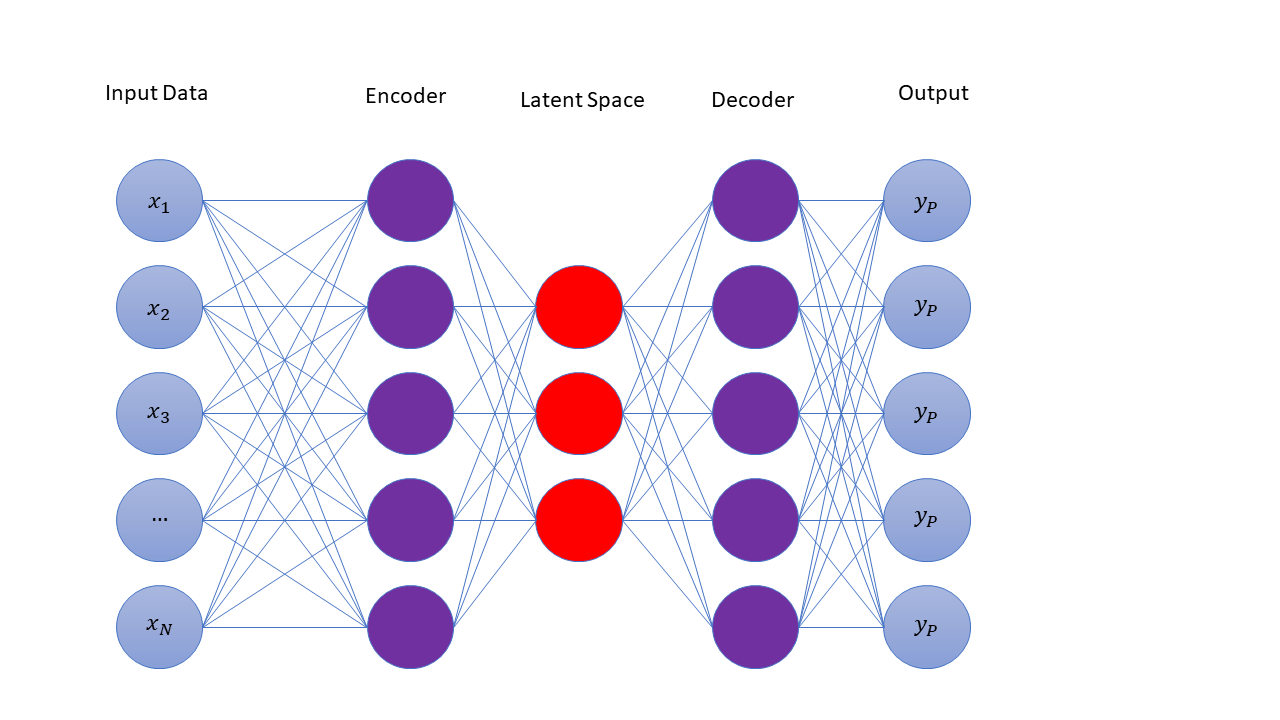
\includegraphics[width=19cm,height=20cm,keepaspectratio]{figures/autoencoder_diagram.png}
    \caption{An autoencoder network composed of two neural networks defined as the encoder 
    and the decoder networks. Here, both networks are represented as fully-connected networks, but could also be any number of other network architectures such \ac{CNN}s and \ac{LSTM} networks. The encoder network takes as input a set of data and compresses the data  
    through a bottleneck called the latent space. The latent space is then given as input to the decoder network which tries to reconstruct the given input $x_1 ... x_N$.}
    \label{fig:autoencoder_diagram}
\end{figure}

\begin{equation}
    l(f(x)) = \sum_k{(f(x)_k - x_k)^2},
\end{equation}

where $f(x)_k$ is the output from the decoder network on the 
kth training/testing sample of the \ac{AE} and $x_k$ is the 
kth training/testing sample. During training, $f(x)_k$ is trained 
to be as similar to $x_k$ as possible in order to minimise 
$l(f(x))$. The lower the value $l(f(x))$ is, the better the network 
is performing. The loss $l(f(x))$ is then backpropagated through 
the network adjusting the weights and biases in order to  
further minimise the loss.

\ac{AE}s can be used across a variety of applications including: 
dimensionality reduction \cite{6910027}, image denoising \cite{NISHIO2017e00393},
feature extraction \cite{7965877} and many others. Although powerful, 
one of the limitations of an \ac{AE} is the way it represents the 
latent space. Within the context of \ac{AE}s as content generators 
the reader would be forgiven for thinking that, if properly trained, 
one could just simply sample from the latent space uniformly 
in order to generate unique content. However, due to the fact 
that the network is not required to distribute learned latent 
space representations during training (features are allowed 
to be encoded anywhere in the latent space), it is not 
guaranteed that latent space samples will be from a 
learned part of the latent space.

%
% Variational autoencoders
%
\subsubsection{Variational Autoencoders}

We can overcome this, through the use of a \ac{VAE} (see illustration in 
Fig.\ref{fig:simple_vae}. 
A \ac{VAE} is nearly identical to an \ac{AE}, except for 
the main differences arising from how the latent space 
is represented and how the loss function is constructed. 
If we go back to our original problem, where the encoder is given 
a sample MNIST digit image; instead of having the encoder network 
output a single predicted value for each dimension in the 
latent space, we now have it output both a predicted 
mean and standard deviation value describing a Gaussian 
for each dimension. Samples are then drawn from the the 
predicted distributions and given as input the decoder network. 
The decoder network produces estimates trying to reconstruct 
the given input to the encoder network. The loss for 
a \ac{VAE} is also slightly different and is represented 
as 

\begin{figure}
    \centering
    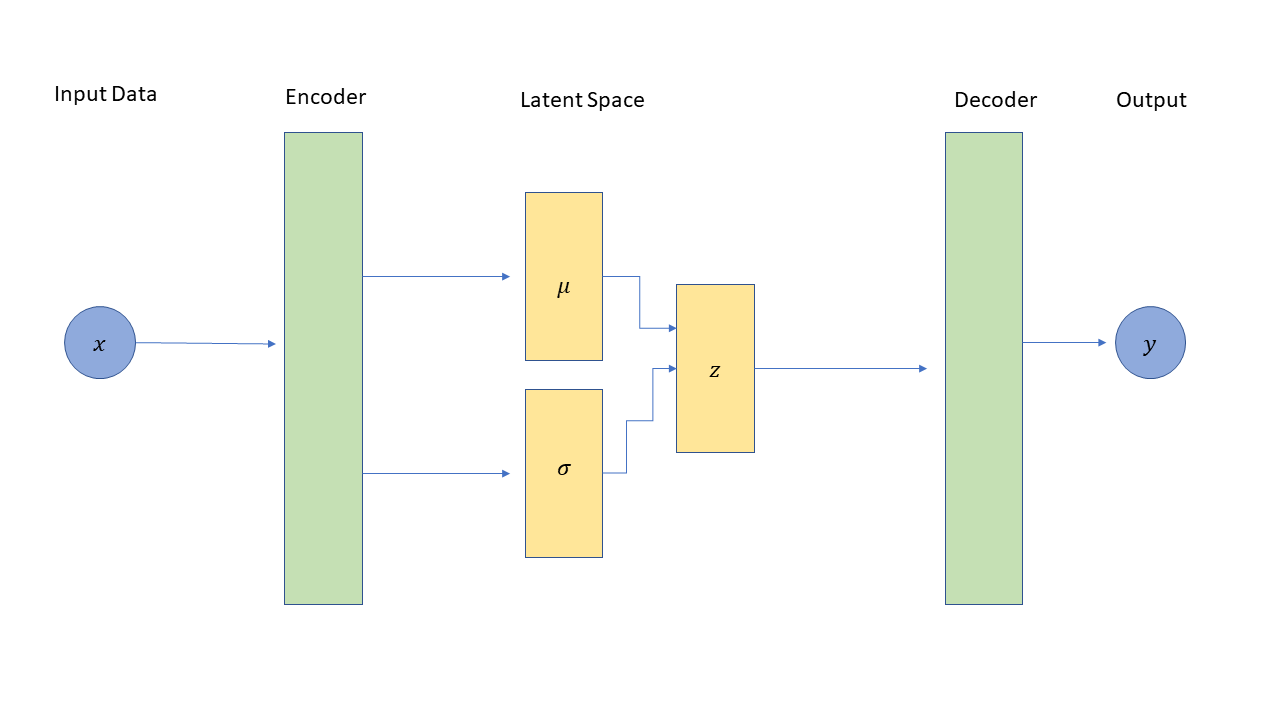
\includegraphics[width=16cm,height=20cm,keepaspectratio]{figures/simple_vae_diagram.png}
    \caption{A simplified diragram of a variational autoencoder network. The input data $x$ is passed to the encoder neural network which produces predictions on the means $\mu$ and standard deviations $\sigma$ of multi-variate Gaussian distributions describing the latent space. Samples are drawn from the predicted distributions $z$ in order to get samples from the latent space. These latent space samples are then passed to the decoder network which attempts to reconstruct the given input $x$.}
    \label{fig:simple_vae}
\end{figure}

\begin{equation}
    l(f(x)) = \sum_k{ (f(x)_k - x_k)^2 + 
    D_{\textrm{KL}}[N(\mu_k, \sigma_k), N(0, 1)]},
\end{equation}

where $f(x_k)$ is the predicted output from the decoder, $x_k$
is the given input to the encoder, $D_{\textrm{KL}}$ is the \ac{KL} divergence 
between latent space samples from predicted Gaussians $N(\mu_k, \sigma_k)$ 
and samples from a mean zero unit variant Gaussian 
distribution $N(0,1)$. 

We can derive this loss function by first assuming that we 
want to approximate the optimal latent space posterior 
representation using a neural network. I will be directly following a 
similar derivation done in \cite{1907.08956}. We can define the 
difference between the approximate and the truth as 

\begin{equation}
    D_{\textrm{KL}}(q_{\theta}(z|x_k) || p(z|x_k)) = -\int q_{\theta}(z|x_k) \log(\frac{p(z|x_k)}{q_{\theta}(z|x_k)}) dz,
\end{equation}

where $q_{\theta}(z|x_k)$ is the approximate posterior of the 
latent space and $p(z|x_k)$ is the optimal representation. 
We can then substitute Bayes theorem in for the truth 
$p(z|x_k)$ as 

\begin{equation}
    D_{\textrm{KL}}(q_{\theta}(z|x_k) || p(z|x_k)) = -\int q_{\theta}(z|x_k) 
    \log(\frac{p(x_k|z) p(z)}{q_{\theta}(z|x_k) p(x_k)}) dz. 
\end{equation}

We now separate out the division using the laws of logarithms and 
distribute the integrand

\begin{equation}
    D_{\textrm{KL}}(q_{\theta}(z|x_k) || p(z|x_k)) = -\int q_{\theta}(z|x_k) 
    \log(\frac{p(x_k|z) p(z)}{q_{\theta}(z|x_k)}) - \log(p(x_k)) dz. 
\end{equation}\

\begin{equation}
    -\int q_{\theta}(z|x_k) 
    \log(\frac{p(x_k|z) p(z)}{q_{\theta}(z|x_k)}) +
    \int q_{\theta}(z|x_k) \log(p(x_k)) dz. 
\end{equation}\

Due to the fact that $q_{\theta}(z|x_k)$ is a probability distribution, 
we can assume that integral of $q_{\theta}(z|x_k)$ is equal to 1, 
further simplifying the equation. We also know that by definition the KL 
divergence must be greater than zero, so we can set the whole 
equation to be greater than or equal to zero

\begin{equation}
    -\int q_{\theta}(z|x_k)
    \log(\frac{p(x_k|z) p(z)}{q_{\theta}(z|x_k)})dz +
    \int \log(p(x_k)) \geq 0. 
\end{equation}\

Since $\log(p(x_k))$ is a constant, we can remove the integrand 
on the right-hand side

\begin{equation}
    -\int q_{\theta}(z|x_k)
    \log(\frac{p(x_k|z) p(z)}{q_{\theta}(z|x_k)})dz +
    \log(p(x_k)) \geq 0.
\end{equation}

Moving the integral over to the right-hand side we get 

\begin{equation}
    \log(p(x_k)) \geq \int q_{\theta}(z|x_k)
    \log(\frac{p(x_k|z) p(z)}{q_{\theta}(z|x_k)})dz.\label{eq:lookbackKL}
\end{equation}

Applying rules of logarithms yet again, we can now expand 
out the above equation into 

\begin{equation}
    \log(p(x_k)) \geq \int q_{\theta}(z|x_k)
    [\log(p(x_k|z)) + \log(p(z)) - \log(q_{\theta}(z|x_k))] dz.
\end{equation}

We can now recognize that the expression on the right 
is equivalent to the expectation value over the log 
terms given as 

\begin{equation}
    \log(p(x_k)) \geq E_{\sim q_{\theta}(z|x_k)} 
    [\log(p(x_k|z)) + \log(p(z)) - \log(q_{\theta}(z|x_k))]
\end{equation}

\begin{equation}
    \log(p(x_k)) \geq E_{\sim q_{\theta}(z|x_k)} 
    [\log(p(x_k,z)) - \log(q_{\theta}(z|x_k))].
\end{equation}

Taking a small look back to equation (\ref{eq:lookbackKL}), 
and using the rules of logarithms we can rewrite it as 

\begin{equation}
    \log(p(x_k)) \geq \int q_{\theta}(z|x_k)
    \log(\frac{p(z)}{q_{\theta}(z|x_k)})dz + 
    q_{\theta}(z|x_k) \log({p(x_k|z)}) dz
\end{equation}

We can now see clearly that the first expression on the 
right-hand side of the above inequality is equivalent to the 
negative \ac{KL} divergence between our approximate latent space 
representation $q_{\theta}(z|x_k)$ and our prior on 
the latent space $p(z)$

\begin{equation}
    \log(p(x_k)) \geq - D_{\textrm{KL}}(q_{\theta}(z|x_k) || p(z)) + 
    q_{\theta}(z|x_k) \log({p(x_k|z)}) dz. 
\end{equation}

Conveniently, we also see that the right most term on the 
right-hand side of the inequality can be approximated as the 
expectation value of the log probability of the data $x_k$ 
given $z$

\begin{equation}
    \log(p(x_k)) \geq - D_{\textrm{KL}}(q_{\theta}(z|x_k) || p(z)) + 
    E_{\sim q_{\theta}(z|x_k)}[ \log({p(x_k|z)})].\label{eq:vae_loss}
\end{equation}

And there we have it, the loss function for the \ac{VAE}! 
The whole expression to the right of the inequality
is typically denoted as the \ac{ELBO} because it puts a 
lower bound on the log likelihood of the data $log(p(x))$. For 
practical purposes, expectation value on the right can be computed analytically 
by performing the mean squared error between predictions on $x_k$ given 
latent space samples from $q_{\theta}(z|x_k)$ and the true 
$x_k$ values give as input to the encoder. The KL term acts to constrain 
the form of the approximate posterior $\log(p(x_k))$ according to 
a chosen prior on the latent space representation $p(z)$ across the whole input 
parameter space. The KL is essentially a regularization factor which helps 
the model to learn a well-formed latent space and reduce the likelihood 
of overfitting to the training data. $p(z)$ is nominally chosen to be 
represented as a mean zero, unit variant Gaussian distribution. Samples 
are drawn from predicted means and standard deviations from the 
encoder $q_{\theta}(z|x_k)$ and samples are also drawn from a unit variant 
Gaussian representative of the prior $p(z)$. We can then 
analytically compute the KL divergence value. The results from the KL 
and the ELBO calculations are then summed together and the whole term is 
minimized through backpropogation.

%
% reparameterization trick
%
\subsubsection{The reparameterization trick}

First proposed by Kingma et al. in their now famous \ac{VAE} 
paper \cite{1312.6114}, the reparameterization trick acts to 
solve a problem that we now have with the above derived loss 
function for the \ac{VAE}. That problem being that we cannot 
backpropagate the gradient computed with respect to the loss through 
a random node. The random node referred to is the latent space node 
given as input to the decoder which we define as 

\begin{equation}
    z = \mu + \sigma,\label{eq:before_repar} 
\end{equation}

where $z$ are samples from our latent space, $\mu$ are predicted means 
describing multivariate Gaussians and $\sigma$ are predicted standard deviations. 
We can prove that the above equation is nondifferentiable by first rewriting 
the expression as an expectation value

\begin{equation}
    E_{p(z)}[f(z)],
\end{equation}

If we then go to compute the gradient of the expectation value 
(which we would normally do when updating the weights in the 
\ac{VAE}), then we get the following expression

\begin{align}
    \nabla_{\theta} E_{p(z)}[f_{\theta}(z)] = \nabla_{\theta} \int p(z) f_{\theta}(z) dz\\ 
    = \int p(z) \nabla_{\theta} f_{\theta}(z) dz\\
    = E_{p(z)}[\nabla_{\theta} f_{\theta}(z)]
\end{align}

where it is shown that the gradient of the expectation value 
of $f(z)$ is equivalent to the expectation value of the gradient 
of $f(z)$, which is easily computed since the probability distribution 
is not a function of weights and biases $\theta$. However, if the probability distribution 
were a function of $\theta$, which it is since the latent space is produced 
by the encoder network which is itself a function of weights $\theta$, then 
we see the following happen when taking the gradient of the 
expectation value

\begin{align}
    \nabla_{\theta} E_{p_{\theta}(z)}[f(z)] = \nabla_{\theta} \int p_{\theta}(z) f_{\theta}(z) dz\\
     = \int \nabla_{\theta}  p_{\theta}(z) f_{\theta}(z) dz\\\
     = \int  p_{\theta}(z) \nabla_{\theta} f_{\theta}(z) dz + \int  f_{\theta}(z) dz \nabla_{\theta} p_{\theta}(z) dz\\
     = E_{p_{\theta}(z)}[ \nabla_{\theta} f_{\theta}(z)] + \int  f_{\theta}(z) dz \nabla_{\theta} p_{\theta}(z) dz\\
\end{align}

Although the first summation term is again easily computed, we now are 
left with a particularly intractable integral on the right-hand side.
Monte Carlo methods do allow us to randomly sample from $p_{\theta}(z)$, but 
they do not guarantee that we may take its gradient. 
We are now left with a bit of problem in how we are expected to compute the integral.
However, if we make a small change to equation (\ref{eq:before_repar}) 
by scaling the standard deviation by a deterministic value, we will 
see how this then solves our intractable integral problem. 

If we parameterize this deterministic value as samples drawn 
from a mean zero, unit variant Gaussian distribution 
$\sim N(0, 1)$ which we will denote as 

\begin{equation}
    \epsilon = N(0, 1).
\end{equation}

Then we can rewrite equation (\ref{eq:before_repar}) as 

\begin{equation}
    z = \mu + \sigma \epsilon.
\end{equation}

we'll now simplify the expression to be a function 
$g$ which is parameterized by $\epsilon$ and $x$, 
where $x$ is representative of $\mu$ and $\sigma$

\begin{equation}
    z = g_{\theta}(\epsilon, x).
\end{equation}

rewriting as an expectation value 

\begin{equation}
    E_{p_{\theta}(z)}[f(z^{(i)})] = E_{p(\epsilon)}[
    f(g_{\theta}(\epsilon, x^{(i)}))].
\end{equation}

Taking the gradient with respect to the weights 
and biases of the network $\theta$ we get 

\begin{align*}
    \nabla_{\theta} E_{p_{\theta}(z)}[f(z^{(i)})] = \nabla_{\theta} E_{p(\epsilon)}[
    f(g_{\theta}(\epsilon, x^{(i)}))]\\
    = E_{p(\epsilon)}[ \nabla_{\theta}
    f(g_{\theta}(\epsilon, x^{(i)}))].
\end{align*}

where we see that indeed we can take the gradient 
of $f(g_{\theta}(\epsilon, x^{(i)}))$ since 
$g_{\theta}(\epsilon, x^{(i)})$ is differentiable 
with respect to $\theta$. We can now just simply 
randomly Monte Carlo sample in order to analytically 
calculate $\nabla_{\theta} E_{p_{\theta}(z)}[f(z^{(i)})]$.

%
% conditional variational autoencoders
%
\subsubsection{Conditional Variational Autoencoders}

Through our rigorous derivations in the previous sections 
we have now formulated a loss function which can be trained 
to maximize the expected log probability of our 
decoder's prediction, while also regularizing its
model for the latent space to a smooth representation. 
However, there are some minor drawbacks to the \ac{VAE} 
which make it unsuitable for some generative tasks. 

For example, if we wanted to train our \ac{VAE} on 
the fashion MNIST dataset \cite{DBLP:journals/corr/abs-1708-07747}, 
a database of digit images representative of various classes 
of fashion items (shoes, shirts, pants), in order to 
generate new images of fashion items we would run into 
a problem. This problem is most clearly illustrated when 
taking a closer look at equation (\ref{eq:vae_loss}). In 
equation (\ref{eq:vae_loss}), it can seen that the encoder 
is solely conditioned on inputs from the training space 
$x_k$, but not on what class/type of image $x_k$ is. Similarly, 
the decoder is solely conditioned on the latent space $z$. In order 
to produce a particular class of input from the decoder, we would have 
to know which part of the latent space each class lives and to then 
draw from the location of the latent space that our class of 
interest resides. Knowledge of class location is infeasible to obtain 
after training because the KL 
divergence term in equation (\ref{eq:vae_loss}) enforces that 
on average across the whole training set that the predicted 
latent space locations are representative 
of a mean zero Gaussian distribution, but does not constrain where 
individual classes of input may reside.

The natural question then arises, is it possible to condition 
the network on classes of interest? It turns out that this is 
possible to do by making a minor update to the 
\ac{VAE} loss in equation (\ref{eq:vae_loss})

\begin{equation}
    \log(p(x_k)) \geq - D_{\textrm{KL}}(q_{\theta}(z|x_k,c) || p(z,c)) + 
    E_{\sim q_{\theta}(z|x_k,c)}[ \log({p(x_k|z,c)})].
\end{equation}

Here, we now condition the encoder $q_{\theta}(z|x_k,c)$ on both 
the training images $x_k$ and the class of said images $c$ (see Fig.\ref{fig:simple_cvae}). In the decoder 
$p(x_k|z,c)$ we condition on samples from the latent space $z$ and the 
class $c$. For classification purposes, the class is usually 
parameterized as a single scalar number which is appended to the input to 
the encoder and decoder networks. Now, if we wanted to use the decoder 
as a fashion image generator, we would only simply need to draw a 
random sample from the latent space, choose a class number, and then 
feed both as inputs to the decoder network. 

\begin{figure}
    \centering
    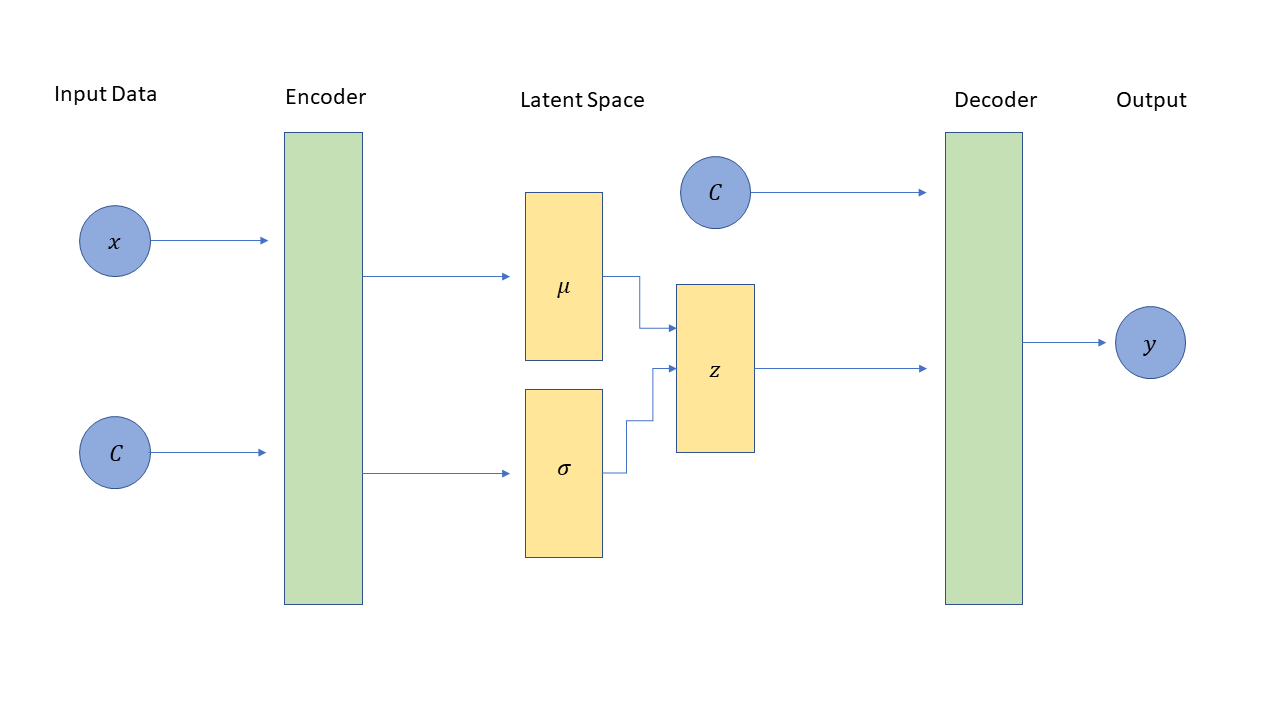
\includegraphics[width=16cm,height=20cm,keepaspectratio]{figures/simple_cvae_diagram.png}
    \caption{A simple \ac{CVAE} diagram consisting of an encoder and decoder network. $x$ data is given as input to the encoder and latent space samples are given as input to the decoder as was the case with the \ac{VAE} diagram in Fig.\ref{fig:simple_vae}. However, now we additionally condition the encoder on the class of $x$ by appending the class label in numerical form to $x$. We also condition the decoder on class $c$ by appending it to the latent space samples $z$.}
    \label{fig:simple_cvae}
\end{figure}